\subsection{Analisi delle ridondanze}
\subsubsection{ridondanza 1}
All'interno dello schema ER è stata identificata 1 ridondanza: la relazione valutazione tra le entità alloggio e recensione. Questa ridondanza ci permette di ottenere le recensioni effettuate su un alloggio utilizzando solamente le entità alloggio e recensione.
La sezione della tavola dei volumi di interesse è:

\small
\setlength\extrarowheight{2pt}
\begin{longtable}{|l|c|c|p{6.3cm}|}
    \hline \textbf{Concetto} & \textbf{Tipo} & \textbf{Volume} & \textbf{Motivazione}                                                                                                                         \\\hline
    \endfirsthead

    \hline \textbf{Concetto} & \textbf{Tipo} & \textbf{Volume} & \textbf{Motivazione}                                                                                                                         \\\hline
    \endhead

    % \hline \multicolumn{4}{|r|}{{Continua all pagina successiva}}                                                                                                                                             \\\hline
    \endfoot

    \endlastfoot
    Alloggio                 & E             & 169.000         & {Ipotizziamo che nella piattaforma verranno registrati circa 169 mila alloggi}                                                               \\\hline
    Prenotazione             & E             & 36.000.000      & {Ipotizziamo che sulla piattaforma siano state effettuate circa 36 milioni di prenotazioni}                                                  \\\hline
    Soggiorno                & E             & 34.920.000      & {Ipotizziamo che sulla piattaforma ci siano stati circa 35 milioni di soggiorni}                                                             \\\hline
    Recensione               & E             & 12.000.000      & {Ipotizziamo che sulla piattaforma vengano scritte circa 12 milioni di recensioni}                                                           \\\hline
    Generazione              & R             & 34.920.000      & {Ipotizziamo che sul totale delle prenotazioni, circa il 2\% vengano cancellate. Tutte le altre diventano soggiorni effettivi}               \\\hline
    Correlazione             & R             & 12.000.000      & {Ipotizziamo che circa 1 soggiorno su 6 riceva una recensione da parte dell'utente o dell'host, e che 1 su 6 la riceva da parte di entrambi} \\\hline
    Riserva                  & R             & 36.000.000      & {Ipotizziamo che tutti gli alloggi vengano riservati circa 36 milioni di volte, una volta per ogni prenotazione}                             \\\hline
    Valutazione              & R             & 2.000.000       & {Ipotizziamo che circa 1 recensione su 3 viene scritta verso un alloggio}                                                                    \\\hline
\end{longtable}
\normalsize

\subsubsection{todo:titoletto}
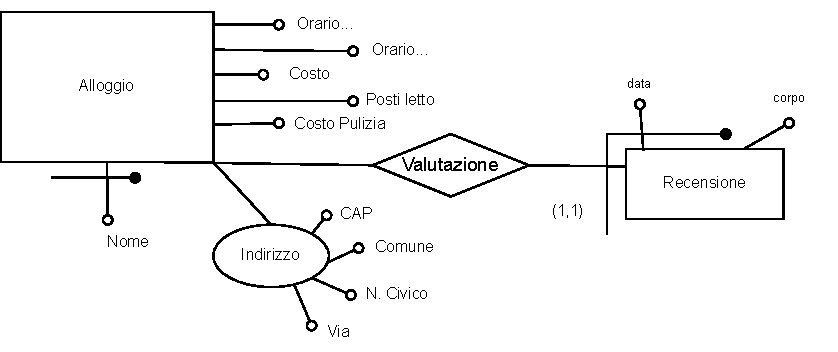
\includegraphics[width=\textwidth]{resources/page5.pdf}

\subsubsection{todo:titoletto}
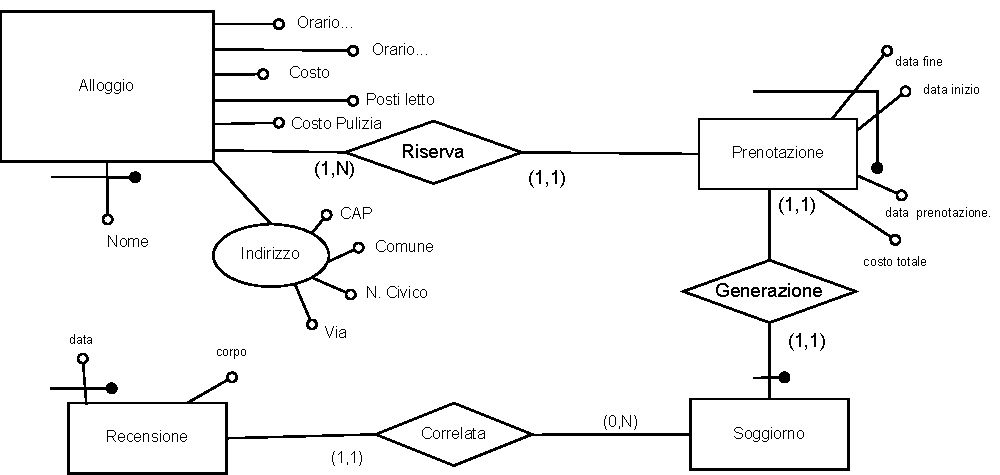
\includegraphics[width=\textwidth]{resources/page6.pdf}

\subsubsection{Tavola degli accessi}
Analizziamo l'operazione "\textbf{Scrittura di una recensione su un alloggio (3000 volte al giorno)}"

\small
\setlength\extrarowheight{2pt}
\begin{longtable}{|lccc|}
    \caption*{In presenza di ridondanza}                                             \\

    \hline \textbf{Concetto} & \textbf{Costrutto} & \textbf{Accessi} & \textbf{Tipo} \\\hline
    \endfirsthead

    \hline \textbf{Concetto} & \textbf{Costrutto} & \textbf{Accessi} & \textbf{Tipo} \\\hline
    \endhead

    \hline \multicolumn{4}{|r|}{{Continua all pagina successiva}}                    \\\hline
    \endfoot

    \hline
    \endlastfoot
    Alloggio                 & E                  & 1                & S             \\%\hline
    Alloggio                 & E                  & 1                & L             \\%\hline
    Recensione               & E                  & 1                & S             \\%\hline
    Valutazione              & R                  & 1                & S             \\%\hline
\end{longtable}
\normalsize

\small
\setlength\extrarowheight{2pt}
\begin{longtable}{|lccc|}
    \caption*{In presenza di ridondanza}                                             \\

    \hline \textbf{Concetto} & \textbf{Costrutto} & \textbf{Accessi} & \textbf{Tipo} \\\hline
    \endfirsthead

    \hline \textbf{Concetto} & \textbf{Costrutto} & \textbf{Accessi} & \textbf{Tipo} \\\hline
    \endhead

    \hline \multicolumn{4}{|r|}{{Continua all pagina successiva}}                    \\\hline
    \endfoot

    \hline
    \endlastfoot
    Alloggio                 & E                  & 1                & L             \\%\hline
    Riserva                  & R                  & 1                & L             \\%\hline
    Prenotazione             & E                  & 1                & L             \\%\hline
    Generazione              & R                  & 1                & L             \\%\hline
    Soggiorno                & E                  & 1                & S             \\%\hline
    Soggiorno                & E                  & 1                & L             \\%\hline
    Correlazione             & R                  & 1                & S             \\%\hline
    Recensione               & E                  & 1                & S             \\%\hline
\end{longtable}
\normalsize


% 
% 
%      TUTTE LE IMMAGINI DI QUESTA PAGINA VANNO MESSE A COPPIE, 2 IMMAGINI PER PAGINA UNA ACCANTO ALL'ALTRA
% 
%

Analisi di complessità in presenza di ridondanza:
\begin{itemize}
    \item In termini di tempo, vegnono effettuati un accesso in lettura e tre accessi in scrittura, quindi 3000 + 3000 * 3 * 2 (contiamo doppi gli accessi in scrittura), per un totale di 21 mila accessi.
    \item In termini di spazio, viene aggiunta una relazione in cui si memorizzano i dati chiave dell'alloggio all'interno dell'entità recensione: ipotizziamo quindi 200 byte per ogni recensione scritta.
          Considerando 200 byte per 2.000.000 di recensioni totali, il costo totale in termini di spazio risulta essere 200 * 2.000.000 (~381.47Mb).
\end{itemize}

Analisi di complessità in assenza di ridondanza:
\begin{itemize}
    \item In In termini di spazio, il costo totale è 0 byte.
    \item In termini di tempo, vegnono effettuati tre accessi in scrittura e cinque accessi in lettura, quindi 3000 * 5 + 3000 * 3 * 2 (contiamo doppi gli accessi in scrittura), per un totale di 33 mila accessi.
\end{itemize}

Dall'analisi effettuata, con l'assenza di ridondanza, risulta un peggioramento nei tempi di accesso (circa il 35\% di tempo in più) ma un risparmio notevole in termini di spreco di memoria: decidiamo per cui di rimuovere la ridondanza.

\subsection{Eliminazione delle generalizzazioni}
\subsubsection{Entità RECENSIONE}
\includegraphics[width=\textwidth]{resources/page7}
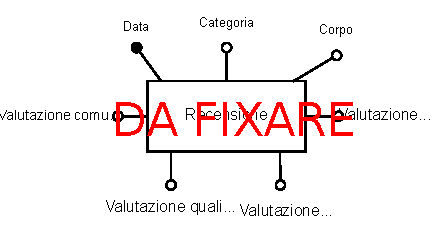
\includegraphics[width=\textwidth]{resources/page8}
La generalizzazione è di tipo totale ed esclusiva.\\
La decisione consiste nel raggruppamento delle entità	figlie nell'attributo categoria. Gli attributi specifici delle entità figlie (valutazioni) vengono spostate nell'entità padre, diventando annullabili. L'attributo categoria sarà un valore not null.

\subsubsection{Entità ALLOGGIO}
\includegraphics[width=\textwidth]{resources/page9}
\clearpage
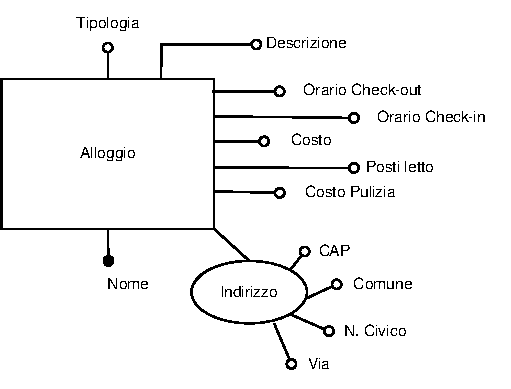
\includegraphics[width=\textwidth]{resources/page10}
La generalizzazione è di tipo totale ed esclusiva. La decisione consiste nel raggruppamento delle entità	figlie nell'attributo tipologia, con valore not null.

\subsubsection{Entità UTENTE}
\includegraphics[width=\textwidth]{resources/page11}
\includegraphics[width=\textwidth]{resources/page12}
La generalizzazione è di tipo totale ed esclusiva. La decisione consiste nel raggruppamento dell'entità figlia nell'attributo host, con valore not null. L'attributo superhost dell'entità figlia viene trasferito al padre.

\subsection{Partizionamento/accorpamento di entità e associazioni}
\includegraphics[width=\textwidth]{resources/page13}
\includegraphics[width=\textwidth]{resources/page14}
La decisione di accorpare le entità PRENOTAZIONE e SOGGIORNO in un'unica entità con attributo soggiorno (di tipo booleano) deriva dal fatto che l'entità SOGGIORNO viene generata dalle prenotazioni con stato "confermata".

\includegraphics[width=\textwidth]{resources/page15}
\includegraphics[width=\textwidth]{resources/page16}
Decidiamo di partizionare l'entità \textbf{UTENTE} estraendo gli attributi \textbf{Telefono} e \textbf{Pagamento}, facendoli diventare rispettivamente una nuova entità \textbf{ALLOGGIO}TELEFONO, associata a \textbf{UTENTE} tramite la relazione \textbf{POSSEDIMENTO}, e una nuova entità \textbf{ALLOGGIO}, associata a \textbf{UTENTE} tramite la relazione \textbf{APPARTENENZA}.

\subsection{Eliminazione degli attributi composti}
L’attributo composto “\textbf{indirizzo}” viene eliminato, considerando i suoi componenti come attributi semplici. Nel caso di indirizzo abbiamo: via, numero civico, cap e comune.
Tale eliminazione viene effettuato nell'entità \textbf{ALLOGGIO}


\subsection{SCHEMA RELAZIONALE}
\begin{itemize}
  \item Utente (\underline{Email}, Nome, Cognome, Password, Host, Superhost)
  \item Telefono (\underline{Utente}, \underline{Numero}, Prefisso)
  \item Pagamento (\underline{Utente}, \underline{Numero}, Circuito)
  \item Utente (\underline{Email}, Nome, Cognome, Password, Host, Superhost)
  \item Alloggio (\underline{ID Alloggio}, Nome, Host, Descrizione, Tipologia, Orario check-in, Orario check-out, Costo, Costo pulizia, Posti letto, CAP, Comune, Civico, Via)
        Alloggio (Host) referenzia Utente (Email)
  \item Prenotazione (\underline{ID Prenotazione}, Richiedente, ID Alloggio, Data inizio, Data fine, Soggiorno, Stato, Numero ospiti)
        Prenotazione (ID Alloggio) referenzia Alloggio (ID Alloggio)
        Prenotazione (Richiedente) referenzia Utente (Email)
  \item Recensione (\underline{ID Recensione}, Autore, ID Prenotazione, Data, Categoria, Valutazione posizione, Valutazione pulizia, Valutazione qualità-prezzo, Valutazione comunicazione, Corpo)
        Prenotazione (Autore) referenzia Utente (Email)
        Prenotazione (ID Prenotazione) referenzia Prenotazione (ID Prenotazione)
  \item Commento (\underline{ ID Commento }, Data, ID Recensione, Autore, Corpo)
        Commento (Autore) referenzia Utente (Email)
        Commento (ID Recensione) referenzia Recensione (ID Recensione)
  \item Lista (\underline{ ID Lista }, Nome, Descrizione, Autore)
        Lista (Autore) referenzia Utente (Email)
  \item Contenuto(\underline{ ID Lista }, \underline{ID Alloggio})
        Contenuto (ID Lista) referenzia Lista (ID Lista)
        Contenuto (ID Alloggio) referenzia Alloggio (ID Alloggio)
\end{itemize}